\documentclass[9pt,twoside]{pnas-new}
% Use the lineno option to display guide line numbers if required.

\articletype{Social Sciences}%%%% Article topic/classification

\templatetype{pnasmathematics} % Choose template
% {pnasresearcharticle} = Template for a two-column research article
% {pnasmathematics} = Template for a one-column mathematics article
% {pnasinvited} = Template for a PNAS invited submission
%\onecolumn

\usepackage{booktabs}

\begin{document}

\title{Household structure, not clinical need, determines who absorbs the cost of long-term care}

% Use letters for affiliations, numbers to show equal authorship (if applicable) and to indicate the corresponding author
\author[a,1]{Alanna Polyak}

\affil[a]{Department of Quantitative Social Science, Dartmouth College, Hanover, NH 03755}

% Please give the surname of the lead author for the running footer
\leadauthor{Polyak}

% Please add a significance statement to explain the relevance of your work
\significancestatement{Most long-term care in the United States is unpaid work done by family members, and it appears in no measure of health spending. Using a nationally representative survey of 2,142 older adults who need help with daily activities, this study asks what determines whether that help comes entirely from relatives rather than from paid providers. The answer is not how sick someone is. Functional limitation and diagnosed neurological disease have small, barely detectable effects, while who a person lives with dominates every model tested. Read against the standard equity criterion for health services, which holds that need should drive utilization, this is a finding about inequity: the households least able to purchase an alternative are the ones absorbing the most unpaid labor.}

% Please include corresponding author, author contribution and author declaration information
\authorcontributions{A.P. designed the study, wrote all analysis code, performed the analysis, and wrote the paper.}
\authordeclaration{The author declares no competing interests.}
\correspondingauthor{\textsuperscript{1}To whom correspondence should be addressed. E-mail: alanna.g.polyak.28\@dartmouth.edu}

% At least three keywords are required at submission. Please provide three to five keywords, separated by the pipe symbol.
\keywords{informal caregiving $|$ long-term care $|$ machine learning $|$ health equity $|$ Health and Retirement Study}

\begin{abstract}
Long-term care in the United States is delivered largely by unpaid family members, a transfer invisible to health expenditure accounting. Using the 2022 Health and Retirement Study, I construct the share of monthly care hours a respondent receives from unpaid informal helpers ($n = 2{,}142$ recipients, $4{,}481$ helper records) and ask what predicts it. The outcome is close to degenerate: 84.7\% of recipients get every hour of their care from family and friends. Comparing ordinary least squares against cross-validated gradient boosting, a fractional-response specification, an explicit two-part model, and a multilayer perceptron, no model class explains more than about a tenth of held-out variance, and the neural network performs worse than predicting the sample mean. Across every specification, household composition dominates: living arrangement carries the largest coefficients and the largest SHAP attributions, while stroke ($\beta = -0.015$, $P = 0.03$) and functional limitation ($\beta = -0.026$, $P = 0.001$) are statistically detectable but small. Interaction tests reveal that care intensity and living alone interact ($\beta = -0.032$, $P = 0.005$), an effect independently recovered as the strongest pairwise SHAP interaction. Two methodological results follow: a two-tier target-leakage failure in network-derived features that inflates held-out $R^2$ from 0.087 to 0.644, and an automated procedure that reconstructs the crosswalk between US and English survey instruments at 71\% top-1 accuracy against a 0.2\% random baseline. All analysis is descriptive; no causal effect is estimated.
\end{abstract}

\dates{This manuscript was compiled on \today}
\doi{\url{www.pnas.org/cgi/doi/10.1073/pnas.XXXXXXXXXX}}

\maketitle
\thispagestyle{firststyle}
\ifthenelse{\boolean{shortarticle}}{\ifthenelse{\boolean{singlecolumn}}{\abscontentformatted}{\abscontent}}{}


\Firstpage

%The \Firstpage command is used to format the first page text column size. The same size will be maintained for subsequent paragraph until the \Endparasplit or \Parasplit command is encountered.


% If your first paragraph (i.e. with the \dropcap) contains a list environment (quote, quotation, theorem, definition, enumerate, itemize...), the line after the list may have some extra indentation. If this is the case, add \parshape=0 to the end of the list environment.
\dropcap{T}he majority of long-term care received by older Americans is not
purchased. It is provided by spouses, adult children and other relatives,
without pay and usually without training \cite{adi2018}. Because this labor
never transacts, it is absent from national health expenditure accounts, and the
households supplying it are invisible to the statistics used to allocate
long-term care policy. The question this paper addresses is distributional: among
older adults who already need help with basic daily activities, what determines
whether that help arrives entirely from family, or whether paid and
institutional providers enter at all?

Three frameworks make competing predictions. Andersen's behavioral model of
health services use partitions determinants into \emph{predisposing}
characteristics, \emph{enabling} resources, and \emph{need}, and supplies the
field's standard equity criterion: in a well-functioning system need should
dominate utilization, and the degree to which enabling resources instead drive
it measures inequity. Cantor's hierarchical compensatory model holds that older
adults draw on a ranked ordering of caregivers---spouse, then adult children,
then other kin, then formal services---turning to each tier only when the
preceding one is exhausted, which predicts that household composition should
dominate. Litwak's task-specific model is the only one of the three that
requires an \emph{interaction}: informal and formal providers are matched to
tasks by comparative advantage, so the effect of rising need should depend on
whether anyone is available in the household to absorb it.

\paragraph{Related work.} Cross-national comparison has established that
caregiving composition varies sharply with the structure of a country's
long-term care system \cite{jang2012}, and microsimulation projects European
informal care demand rising through 2050 \cite{cattaneo2025}. Work closest to
this study examines how caregiving for adults with cognitive decline is
distributed within and beyond the household \cite{geronb2025}. This paper
extends that literature in three ways. First, it treats the informal share as a
continuous bounded outcome rather than a binary caregiver-present indicator, and
shows that the resulting spike at one has consequences for model choice that the
existing literature does not address. Second, it compares five model families
under a design that respects household clustering, rather than reporting a
single specification. Third, it treats the failure modes---leakage, a
non-surviving hypothesis, an automated harmonization that fails confidently---as
results in their own right.\Endparasplit

%The \Endparasplit command is used to end the formatting of the text column size that was set by the \Firstpage command. This will restore the default column size for the subsequent text.
%
%The \Parasplit command should be used if the page ends in the middle of a paragraph, allowing the column formatting to continue seamlessly on the next page.

% Note: please start your introduction without including the word ``Introduction'' as a section heading (except for math articles in the Physical Sciences section); this heading is implied in the first paragraphs.

\section*{Data}

\paragraph{Source and window.} The Health and Retirement Study is a nationally
representative biennial panel of US adults over 50 and their spouses, fielded by
the Survey Research Center at the University of Michigan. This analysis uses the
2022 Core final release together with the 2022 Tracker file. The 2022 wave
contains 15,787 respondent records collected by in-person, telephone and web
interview, with proxy interviews taken where a respondent could not self-report.
Proxy status matters here because cognitive impairment is simultaneously a
predictor of interest and a cause of proxy interviewing.

\paragraph{Unit of analysis.} The original data are supplied at two levels. The
respondent-level file records difficulty with six activities of daily living
(ADLs: dressing, walking, bathing, eating, transferring, toileting) and five
instrumental activities (IADLs: meal preparation, shopping, telephone use,
medication management, money management). The \emph{helper-level} file records
one row per person who helps the respondent, carrying that helper's relationship,
days of help per month, hours per helping day, whether insurance pays them, and
out-of-pocket payment. The unit of analysis in this paper is the
\emph{respondent}; helper records are aggregated up.

\paragraph{Outcome construction.} For each helper record, monthly care hours are
days of help multiplied by hours per helping day, reconciling the three ways HRS
permits the frequency question to be answered. A helper is classified as
\emph{formal} if the relationship is an organization, an institutional employee,
a paid helper, a professional or an online service, and as \emph{informal}
otherwise---except that informal helpers whom the household reports paying out of
pocket are reclassified as formal. That rule matters substantively: a daughter
being paid to provide care is performing paid work, and counting her as informal
would understate the market's role. Summing within respondent gives
\begin{equation}
\label{eq:outcome}
s_i = \frac{\sum_{j \in \mathcal{I}_i} h_{ij}}{\sum_{j \in \mathcal{H}_i} h_{ij}},
\end{equation}
where $\mathcal{H}_i$ is the set of helpers for respondent $i$, $\mathcal{I}_i
\subseteq \mathcal{H}_i$ the informal subset, and $h_{ij}$ monthly hours. After
restricting to respondents aged 50 and over with usable hours data, the analysis
sample is $n = 2{,}142$ with 33 base predictors.

\paragraph{Missingness.} HRS encodes ``don't know'' and ``refused'' as reserved
numeric values (8/9, 98/99, $-8$); these are converted to missing per variable
rather than read as data. For every predictor with more than 1\% missingness a
binary indicator is created before median imputation. This is deliberate rather
than conventional. Allowing a gradient-boosted model to route missing values
down its own default branches would fold the \emph{fact} of missingness into the
SHAP attribution of the parent feature, which misleads when missingness is not
at random---and here it plainly is not. The word-recall test is missing for 21\%
of the sample, and missing precisely among the cognitively impaired and
proxy-interviewed respondents whose care arrangements are most distinctive.

\paragraph{Limitations of the source.} Four are material. The design is
cross-sectional, so nothing here speaks to how arrangements evolve as need
progresses. Survey weights are available for only 80.3\% of the sample, and
critically for none of the 73 nursing-home residents, because HRS respondent
weights are constructed for the community-dwelling population; any weighted
analysis therefore silently drops institutionalized respondents. Section~G asks
about helpers who assist the respondent personally, and facility staff appear
under-reported relative to family visits, which produces a counterintuitive
positive association between nursing-home residence and the informal share.
Finally, the outcome is constructed from the helper roster, so any feature
derived from that roster is downstream of the outcome---a point returned to
below.

\section*{Methods}

\paragraph{Cleaning.} \texttt{code/00\_build\_analysis\_file.py} performs every
cleaning step. HRS reserved codes for ``don't know'' and ``refused'' are mapped
to missing before any arithmetic, via \texttt{clean\_codes} in
\texttt{utils.py}; leaving them in place would enter values such as 998 into an
hours total. Helper records with no usable hours or no relationship code are
dropped (4{,}481 records to 3{,}666). Helpers paid out of pocket by the family
are reclassified from informal to formal, because the analytic distinction is
whether the household bears the cost, not whether the helper is a relative.

\paragraph{Merging.} Three joins, all \textbf{exact on the composite key
(HHID, PN)}, which uniquely identifies a respondent in HRS; no fuzzy matching is
used anywhere. The helper file is aggregated to respondent level and
\textbf{inner joined} to the respondent file, then \textbf{left joined} to the
tracker file for survey weights and household identifiers. The script prints row
counts before and after each join. Table~\ref{tab:sample} reports the resulting
attrition.

\paragraph{Variable definitions.} The outcome is
\begin{equation}
\label{eq:outcome}
s_i \;=\; \frac{\sum_{h \in \mathcal{I}_i} \text{hours}_{ih}}{\sum_{h \in \mathcal{H}_i} \text{hours}_{ih}},
\end{equation}
where $\mathcal{H}_i$ is respondent $i$'s full helper roster and
$\mathcal{I}_i \subseteq \mathcal{H}_i$ the unpaid informal helpers, so
$s_i \in [0,1]$. Predictors fall into four blocks: demographics (age, sex, years
of schooling, race); household structure (lives alone, with partner, with
relative; number of children); clinical need (ADL count, IADL count,
self-rated health, stroke, dementia, word recall, memory rating); and care
intensity (total monthly hours, number of helpers).

\paragraph{Train-test split and validation.} Two schemes are reported because
they disagree. A single \textbf{25\% held-out split} (\texttt{random\_state} =
20260818) is used in \texttt{code/02\_baseline\_ols\_vs\_gbm.py} for the
model-family comparison, with booster hyperparameters selected by an inner
five-fold grid search on the training portion only, so the test split is touched
once. All other performance figures use \textbf{five-fold cross-validation
grouped on household}, which is the design adopted from
\texttt{code/04\_weights\_and\_clustered\_cv.py} onward. Every random seed is
fixed at 20260818.

\paragraph{Identification.} This is a \textbf{descriptive and predictive}
analysis. There is no randomization, instrument or discontinuity, and living
arrangement is plainly not randomly assigned; it is as plausibly a consequence
of care need as a determinant of how that need is met. No causal effect is
estimated or implied anywhere in this paper.

\paragraph{Design.} All held-out performance is estimated by five-fold
cross-validation grouped on household, so that no household spans the
train/test boundary. Spouses are both interviewed in HRS, and 5.3\% of
households contribute more than one respondent, covering about 10\% of rows.
Standard errors on interaction coefficients are clustered on household to match.

\paragraph{Model families.} Five specifications are compared on identical folds
and identical features: (i) ordinary least squares on standardized predictors;
(ii) a gradient-boosted regressor (XGBoost) with depth, tree count, shrinkage
and minimum child weight selected by nested five-fold cross-validation on the
training split; (iii) a fractional-response GLM with a binomial family and logit
link, which uses the binomial likelihood as a quasi-likelihood and guarantees
predictions inside $[0,1]$; (iv) an explicit two-part model, a logit for whether
any formal care is present followed by a conditional model for the share among
those who use some, with combined prediction
\begin{equation}
\label{eq:twopart}
\mathbb{E}[s_i \mid x_i] = \bigl(1 - \pi(x_i)\bigr)\cdot 1
                          + \pi(x_i)\,\mathbb{E}[s_i \mid s_i < 1, x_i],
\end{equation}
where $\pi(x_i) = \Pr(s_i < 1 \mid x_i)$; and (v) a multilayer perceptron with
architecture and $L_2$ penalty selected by grid search.

The fractional-response specification models the conditional mean directly
through a logit link,
\begin{equation}
\label{eq:frac}
\mathbb{E}[s_i \mid x_i] \;=\; \Lambda(x_i^{\top}\beta)
\;=\; \frac{\exp(x_i^{\top}\beta)}{1 + \exp(x_i^{\top}\beta)},
\end{equation}
estimated by maximizing the Bernoulli quasi-likelihood
$\sum_i \{s_i \log \Lambda(x_i^{\top}\beta) + (1-s_i)\log[1-\Lambda(x_i^{\top}\beta)]\}$.
The estimator stays consistent for $\beta$ even though $s_i$ is a proportion
rather than a binary outcome, and predictions are confined to $(0,1)$ by
construction.

\paragraph{Interpretation.} Linear models are interpreted through standardized
coefficients with 95\% confidence intervals; tree models through SHAP values,
which decompose each individual prediction into per-feature contributions.
These are different quantities---a coefficient is a partial effect identical for
every respondent, a SHAP value is a marginal contribution that varies across
them---and the paper treats their disagreement as informative rather than as
error. Pairwise SHAP interaction values are used to detect interactions the
model used, alongside pre-specified product terms.

\section*{Results}

\paragraph{The analysis sample.} Table~\ref{tab:sample} characterizes it and
records where each step of attrition occurs.

\begin{table}[t!]
\centering
\caption{Construction of the analysis sample, HRS 2022 Core. Each row is the
count surviving that step. The largest single loss is helper records missing
usable hours or a relationship code, which cannot contribute to the outcome in
Eq.~\ref{eq:outcome}. Respondents receiving no measurable care hours are dropped
because the outcome is undefined at a zero denominator, not because they are
uninformative.}
\label{tab:sample}
\begin{tabular}{lr}
\toprule
Step & $n$ \\
\midrule
Helper records in HRS 2022 Section G & 4{,}481 \\
\quad with usable hours and relationship & 3{,}666 \\
Respondents represented & 2{,}425 \\
\quad with total care hours $> 0$ & 2{,}161 \\
\quad aged 50+, merged to covariates & \textbf{2{,}142} \\
\bottomrule
\end{tabular}

\addtabletext{Single survey wave, fielded 2022. Analysis sample 2{,}142
respondents; 15.4\% are proxy interviews and 73 are nursing-home residents who
carry no survey weight.}
\end{table}

\subsection*{The outcome is nearly degenerate}

Figure~\ref{fig:outcome} establishes the constraint that governs everything
after it. Of respondents receiving any help, 84.7\% receive every hour of it
from unpaid family and friends; 5.9\% receive none informally; the intermediate
range is nearly empty. Median care intensity is 52 hours per month with a long
right tail, and respondents have on average 1.7 helpers. Care arrangements in
this population are close to binary---either the family absorbs the entire load
or formal providers are involved---and there is correspondingly little variance
for any model to explain.

\begin{figure}[tbhp]
\centering
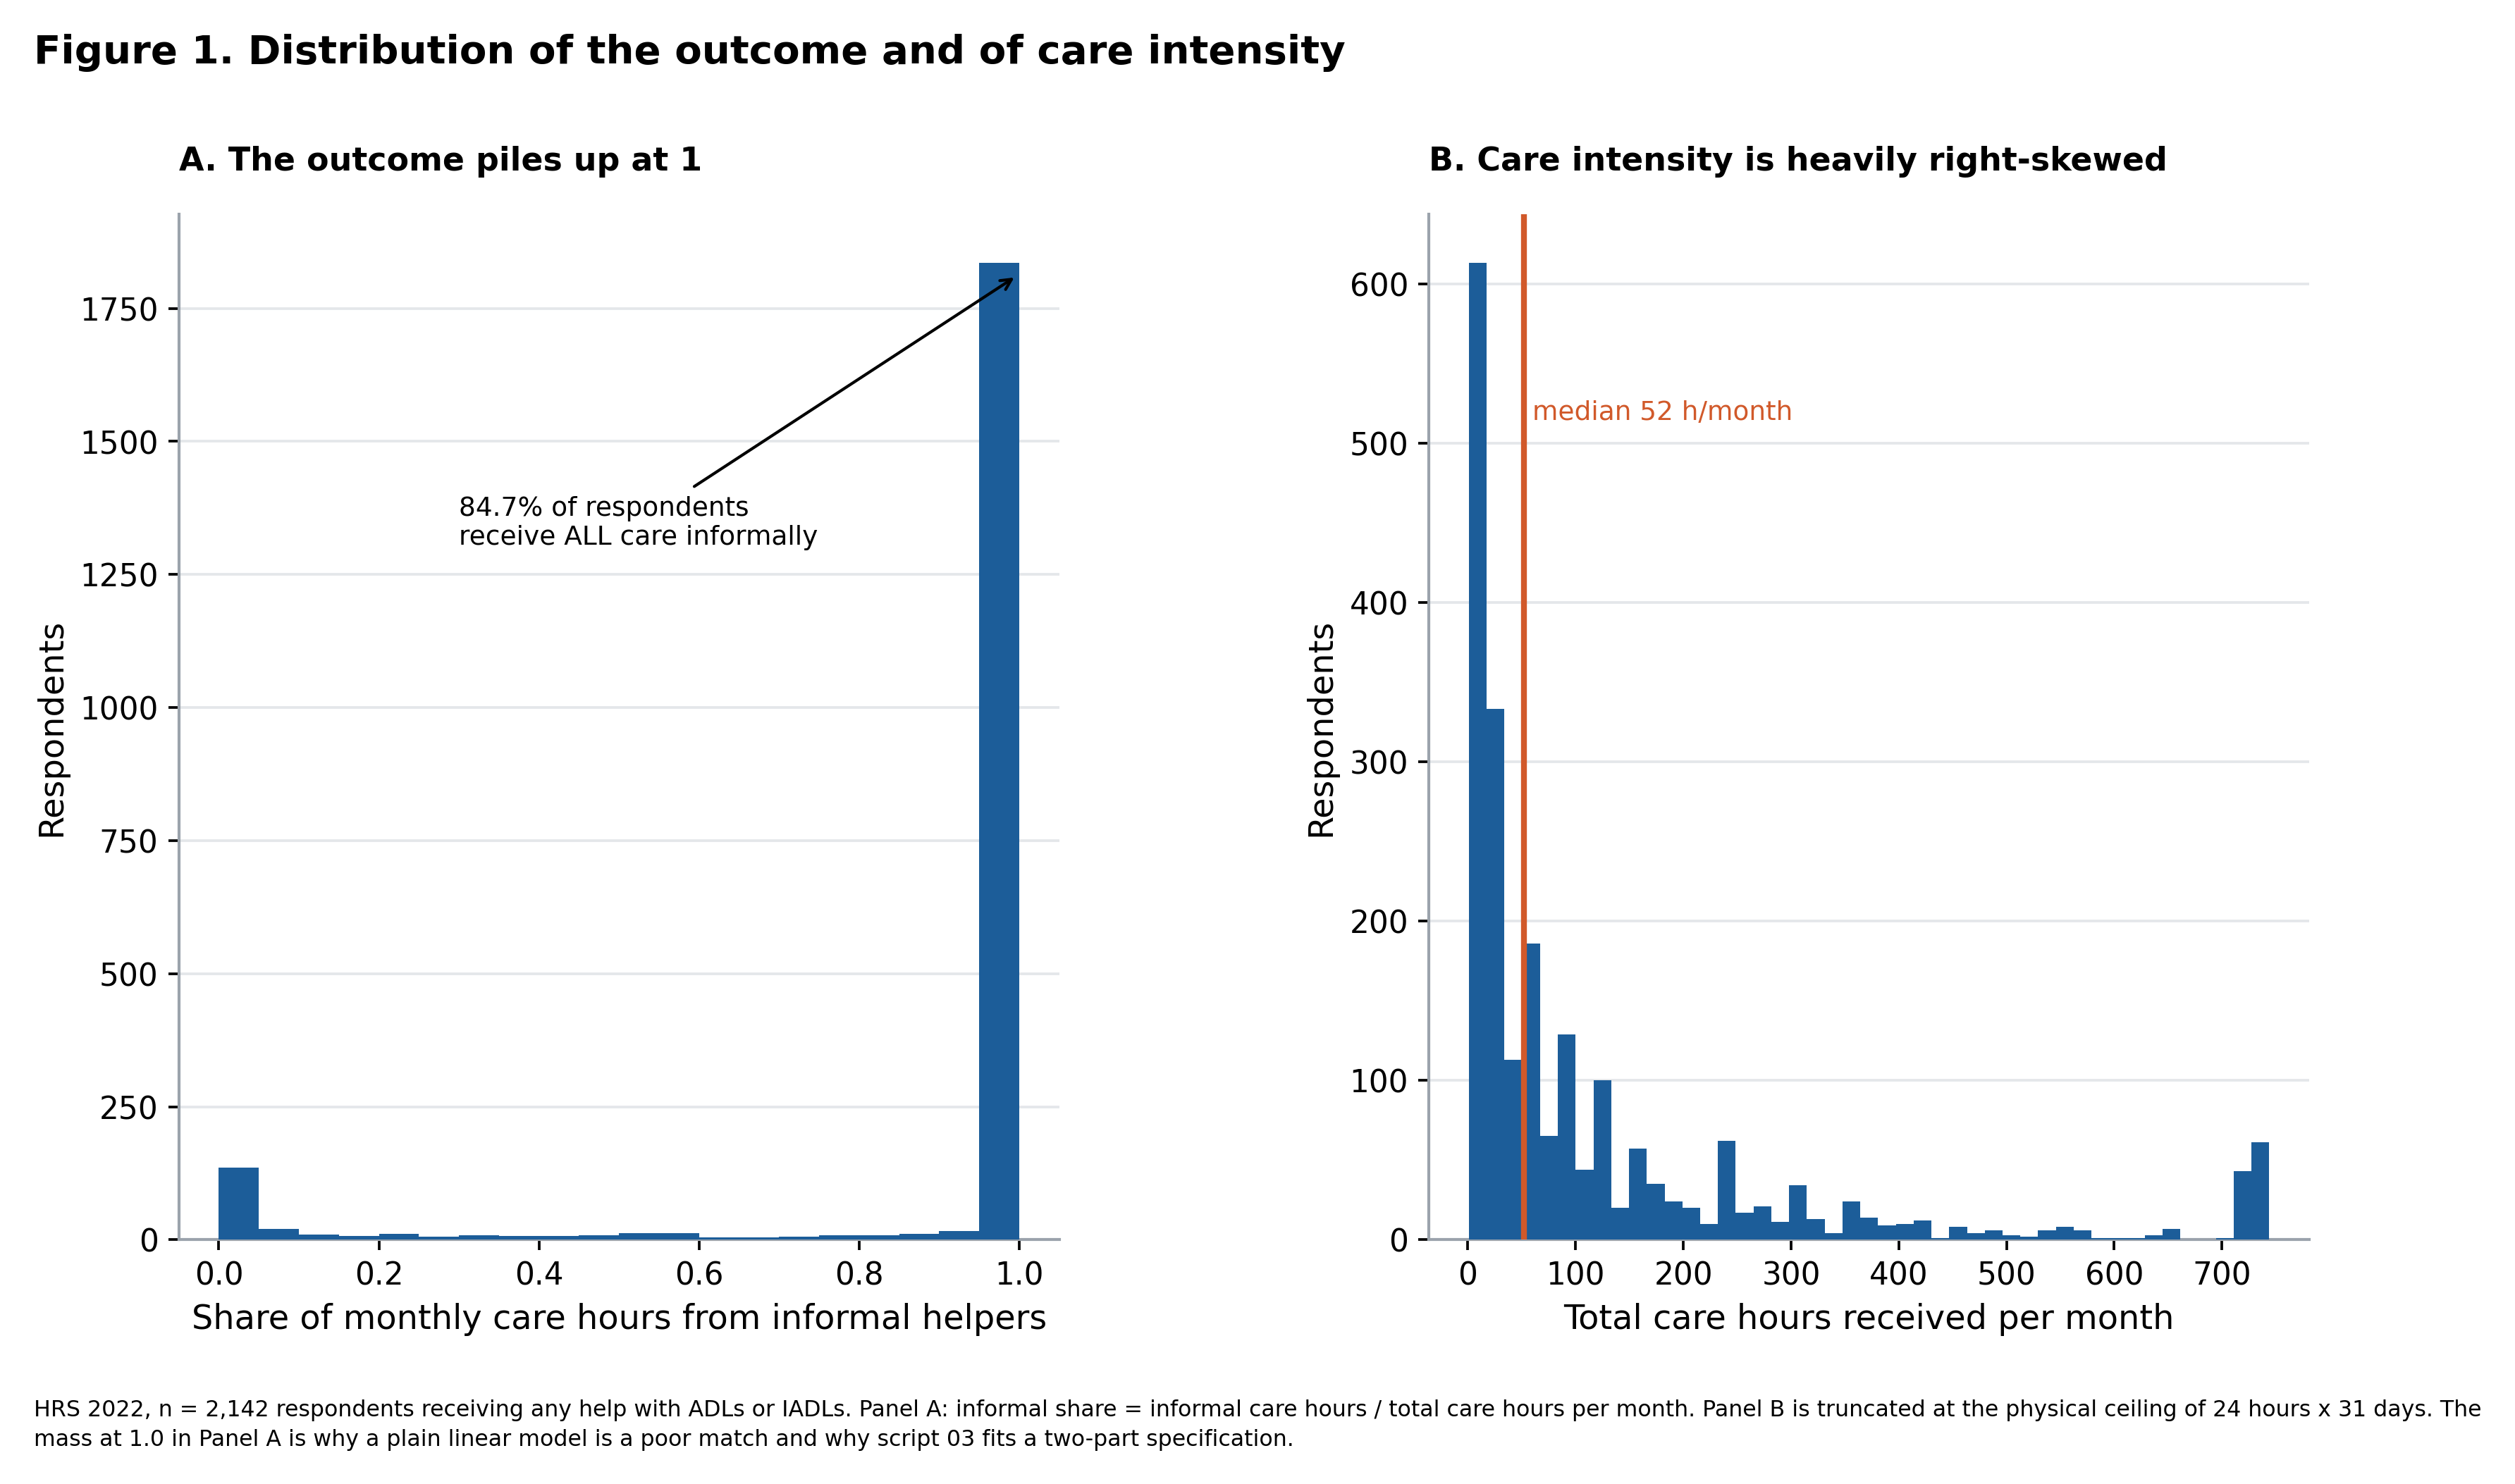
\includegraphics[width=0.80\linewidth]{figures/f01_outcome_and_intensity.png}
\caption{Distribution of the informal care share and of care intensity.
HRS 2022, $n = 2{,}142$ respondents receiving any help with ADLs or IADLs.}
\label{fig:outcome}
\end{figure}

Daughters are the modal caregiver (1,100 helper records), ahead of spouses and
partners (924) and sons (577); paid helpers account for 243. Daughters outnumber
sons roughly two to one, a gendered pattern the hierarchical compensatory model
does not itself predict.

\subsection*{Household structure dominates clinical need}

The mean informal share declines from 0.928 among respondents with no ADL
limitations to 0.837 among those with four, then flattens and partially
reverses: the most severely limited respondents are \emph{not} the most likely
to have formal help. Respondents with a stroke, dementia or Alzheimer's
diagnosis have a mean informal share of 0.888 against 0.900 for those without---a
difference of roughly one percentage point.

Against this, living arrangement carries the largest effects in every
specification. In the linear model, living with a partner
($\beta = +0.061$, $P = 0.006$) and living with a relative
($\beta = +0.046$, $P = 0.012$) are the largest coefficients, while ADL count
($\beta = -0.026$, $P = 0.001$) and stroke ($\beta = -0.015$, $P = 0.032$) are
detectable but an order of magnitude smaller. Read through Andersen's
framework this is an equity result rather than a null one: enabling structure,
not need, is allocating care.

\subsection*{Coefficients and SHAP disagree, for identifiable reasons}

The Spearman correlation between the OLS importance ranking and the SHAP ranking
is $\rho = 0.157$ (Fig.~\ref{fig:forest}). Two features drive the disagreement.
Living alone ranks first by SHAP and 24th by coefficient magnitude, because the
three living-arrangement indicators nearly partition the sample: in the linear
model they compete for a shared signal against an omitted reference category and
the coefficient mass distributes arbitrarily among them, while the tree splits on
whichever single indicator separates best and credits that one. Total care hours
ranks second by SHAP and 31st of 33 by coefficient, because its relationship to
the outcome is non-monotone---very low-intensity help is almost always informal,
very high-intensity help skews formal, the middle is mixed---so a single linear
slope averages to nearly nothing while the tree captures it with a few splits.

\begin{figure}[tbhp]
\centering
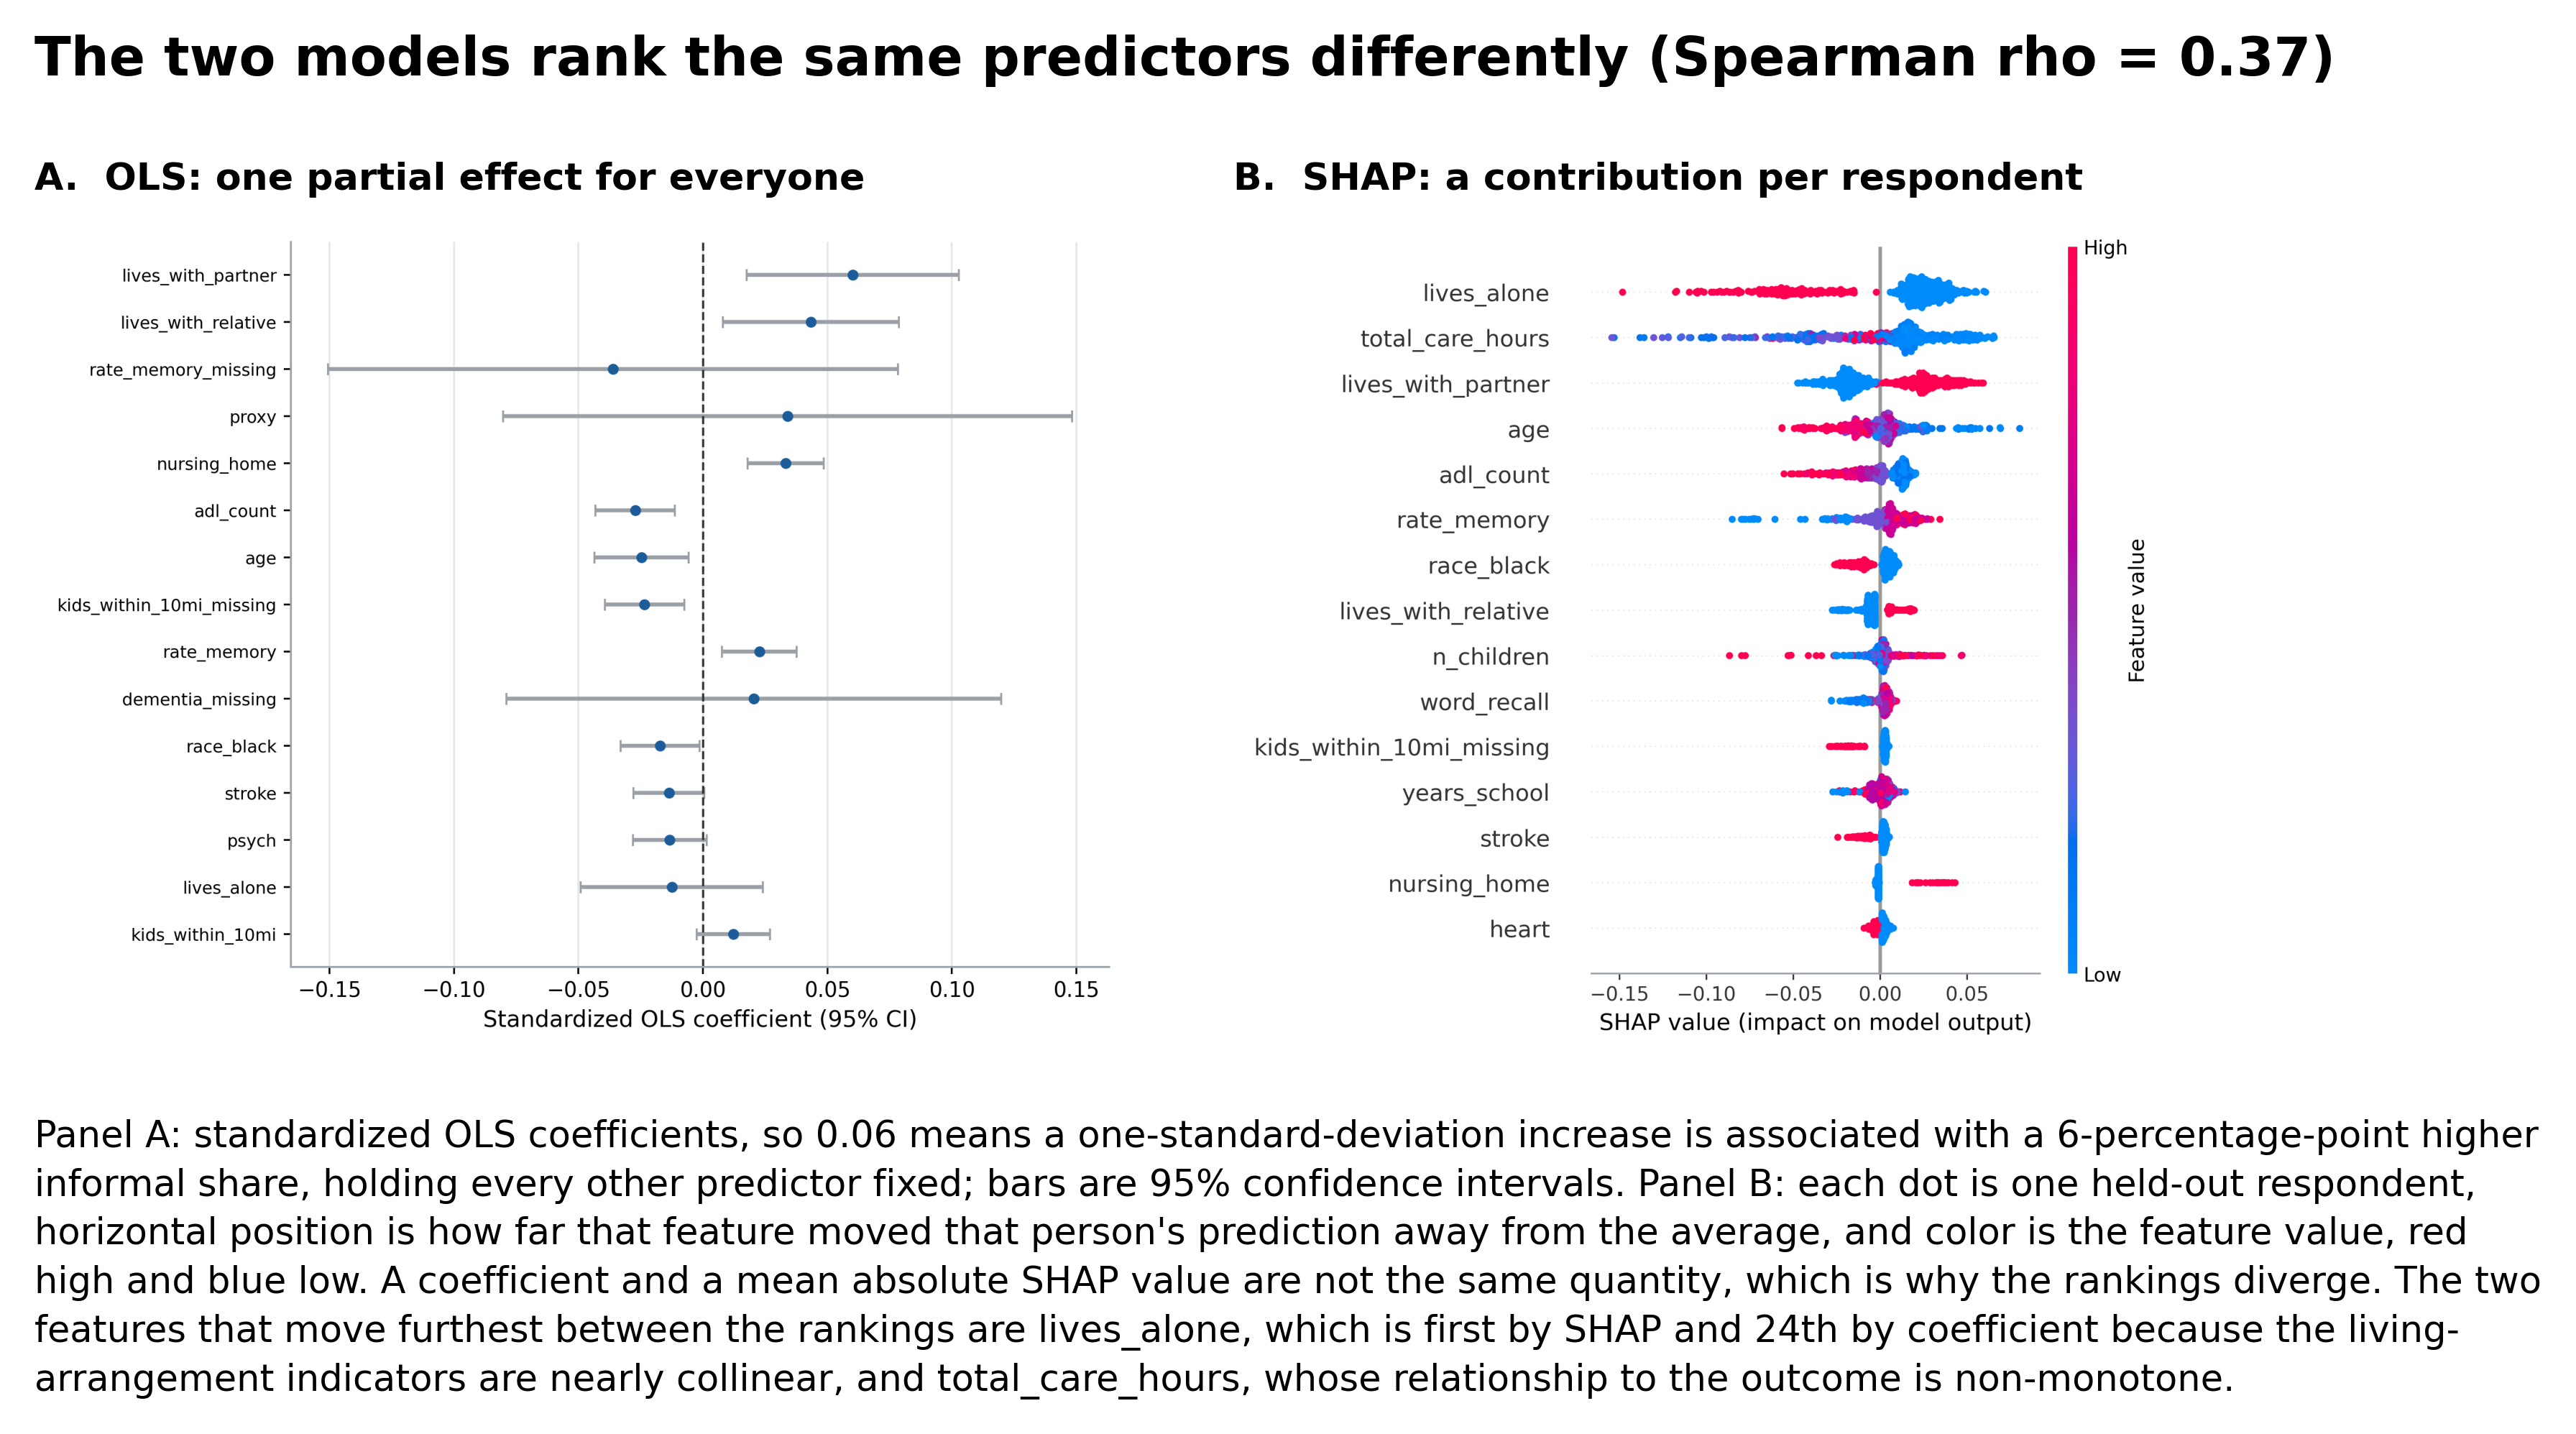
\includegraphics[width=0.80\linewidth]{figures/f04_forest_vs_shap.png}
\caption{Standardized OLS coefficients with 95\% confidence intervals against
the SHAP beeswarm for the tuned gradient-boosted regressor. The two methods
rank the same predictors differently ($\rho = 0.37$).}
\label{fig:forest}
\end{figure}

\subsection*{No model class does well, and the neural network does worst}

Table~\ref{tab:models} reports both evaluation schemes, because they disagree.
On a single 25\% split gradient boosting reaches $R^2 = 0.039$ against 0.011 for
OLS; under household-grouped five-fold cross-validation the booster reaches
0.087 and a ridge model 0.061. A single split on 2{,}142 rows with an 85\% point
mass is optimistic about the gap between model classes and pessimistic about
their level. Tuning does the work: an untuned booster scores $-0.053$, worse
than predicting the mean, so reporting only the tuned figure would misrepresent
boosting as reliably superior at this sample size.

\begin{table}[tbhp]
\centering
\caption{Held-out performance; regression scored by $R^2$, classifiers by AUC.
The lower panel uses five-fold cross-validation grouped on household, so a
married couple never straddles the train and test sets. No model class explains
more than about a tenth of the variance in the informal care share.}
\label{tab:models}
\begin{tabular}{lcc}
\toprule
Model & Task & Held-out \\
\midrule
\multicolumn{3}{l}{\emph{Single 25\% held-out split}} \\
Intercept only            & informal share & $-0.007$ \\
OLS                       & informal share & $0.011$ \\
XGBoost, untuned defaults & informal share & $-0.053$ \\
XGBoost, CV-tuned         & informal share & $\mathbf{0.039}$ \\
Fractional logit          & informal share & $0.032$ \\
Two-part model            & informal share & $\mathbf{0.035}$ \\
Logistic regression       & any formal care & $0.710$ \\
XGBoost classifier        & any formal care & $\mathbf{0.728}$ \\
\midrule
\multicolumn{3}{l}{\emph{Five-fold CV, grouped on household}} \\
XGBoost, CV-tuned         & informal share & $\mathbf{0.087}$ \\
Ridge (linear)            & informal share & $0.061$ \\
Intercept only            & informal share & $-0.000$ \\
Multilayer perceptron     & informal share & $-0.001$ \\
\bottomrule
\end{tabular}
\end{table}

The multilayer perceptron scores below the intercept-only baseline. An
architecture search over seven configurations from a
single eight-unit layer to three stacked layers finds no configuration that
beats the mean, and the best is the smallest. An $L_2$ sweep over five penalties
points the same way: cross-validated performance improves monotonically as the
penalty rises toward the linear limit, from $-0.17$ at $\alpha = 10^{-4}$ to
$-0.001$ at $\alpha = 1$. Both are the signature of a model with far more
parameters than 2{,}142 rows can identify.

The result was predicted before fitting, which is what makes it informative.
Boosted trees are the default on small tabular data; neural networks earn their
keep on high-dimensional structured inputs, none of which is present here.

\subsection*{A bounded outcome needs a bounded likelihood}

OLS produces 58 held-out predictions outside $[0,1]$, which are not
interpretable as shares. Both the fractional logit and the two-part model of
Eq.~\ref{eq:twopart} are constrained by construction and produce none, at
comparable predictive accuracy (Fig.~\ref{fig:twopart}). Decomposing the
two-part model is informative in itself: the first stage, predicting whether any
formal care is present, reaches AUC 0.710 and is well calibrated, while the
second stage---how much of the load formal care takes once present---is close to
unpredictable from these covariates. The covariates tell you whether the market
enters, not how far it goes.

\begin{figure}[tbhp]
\centering
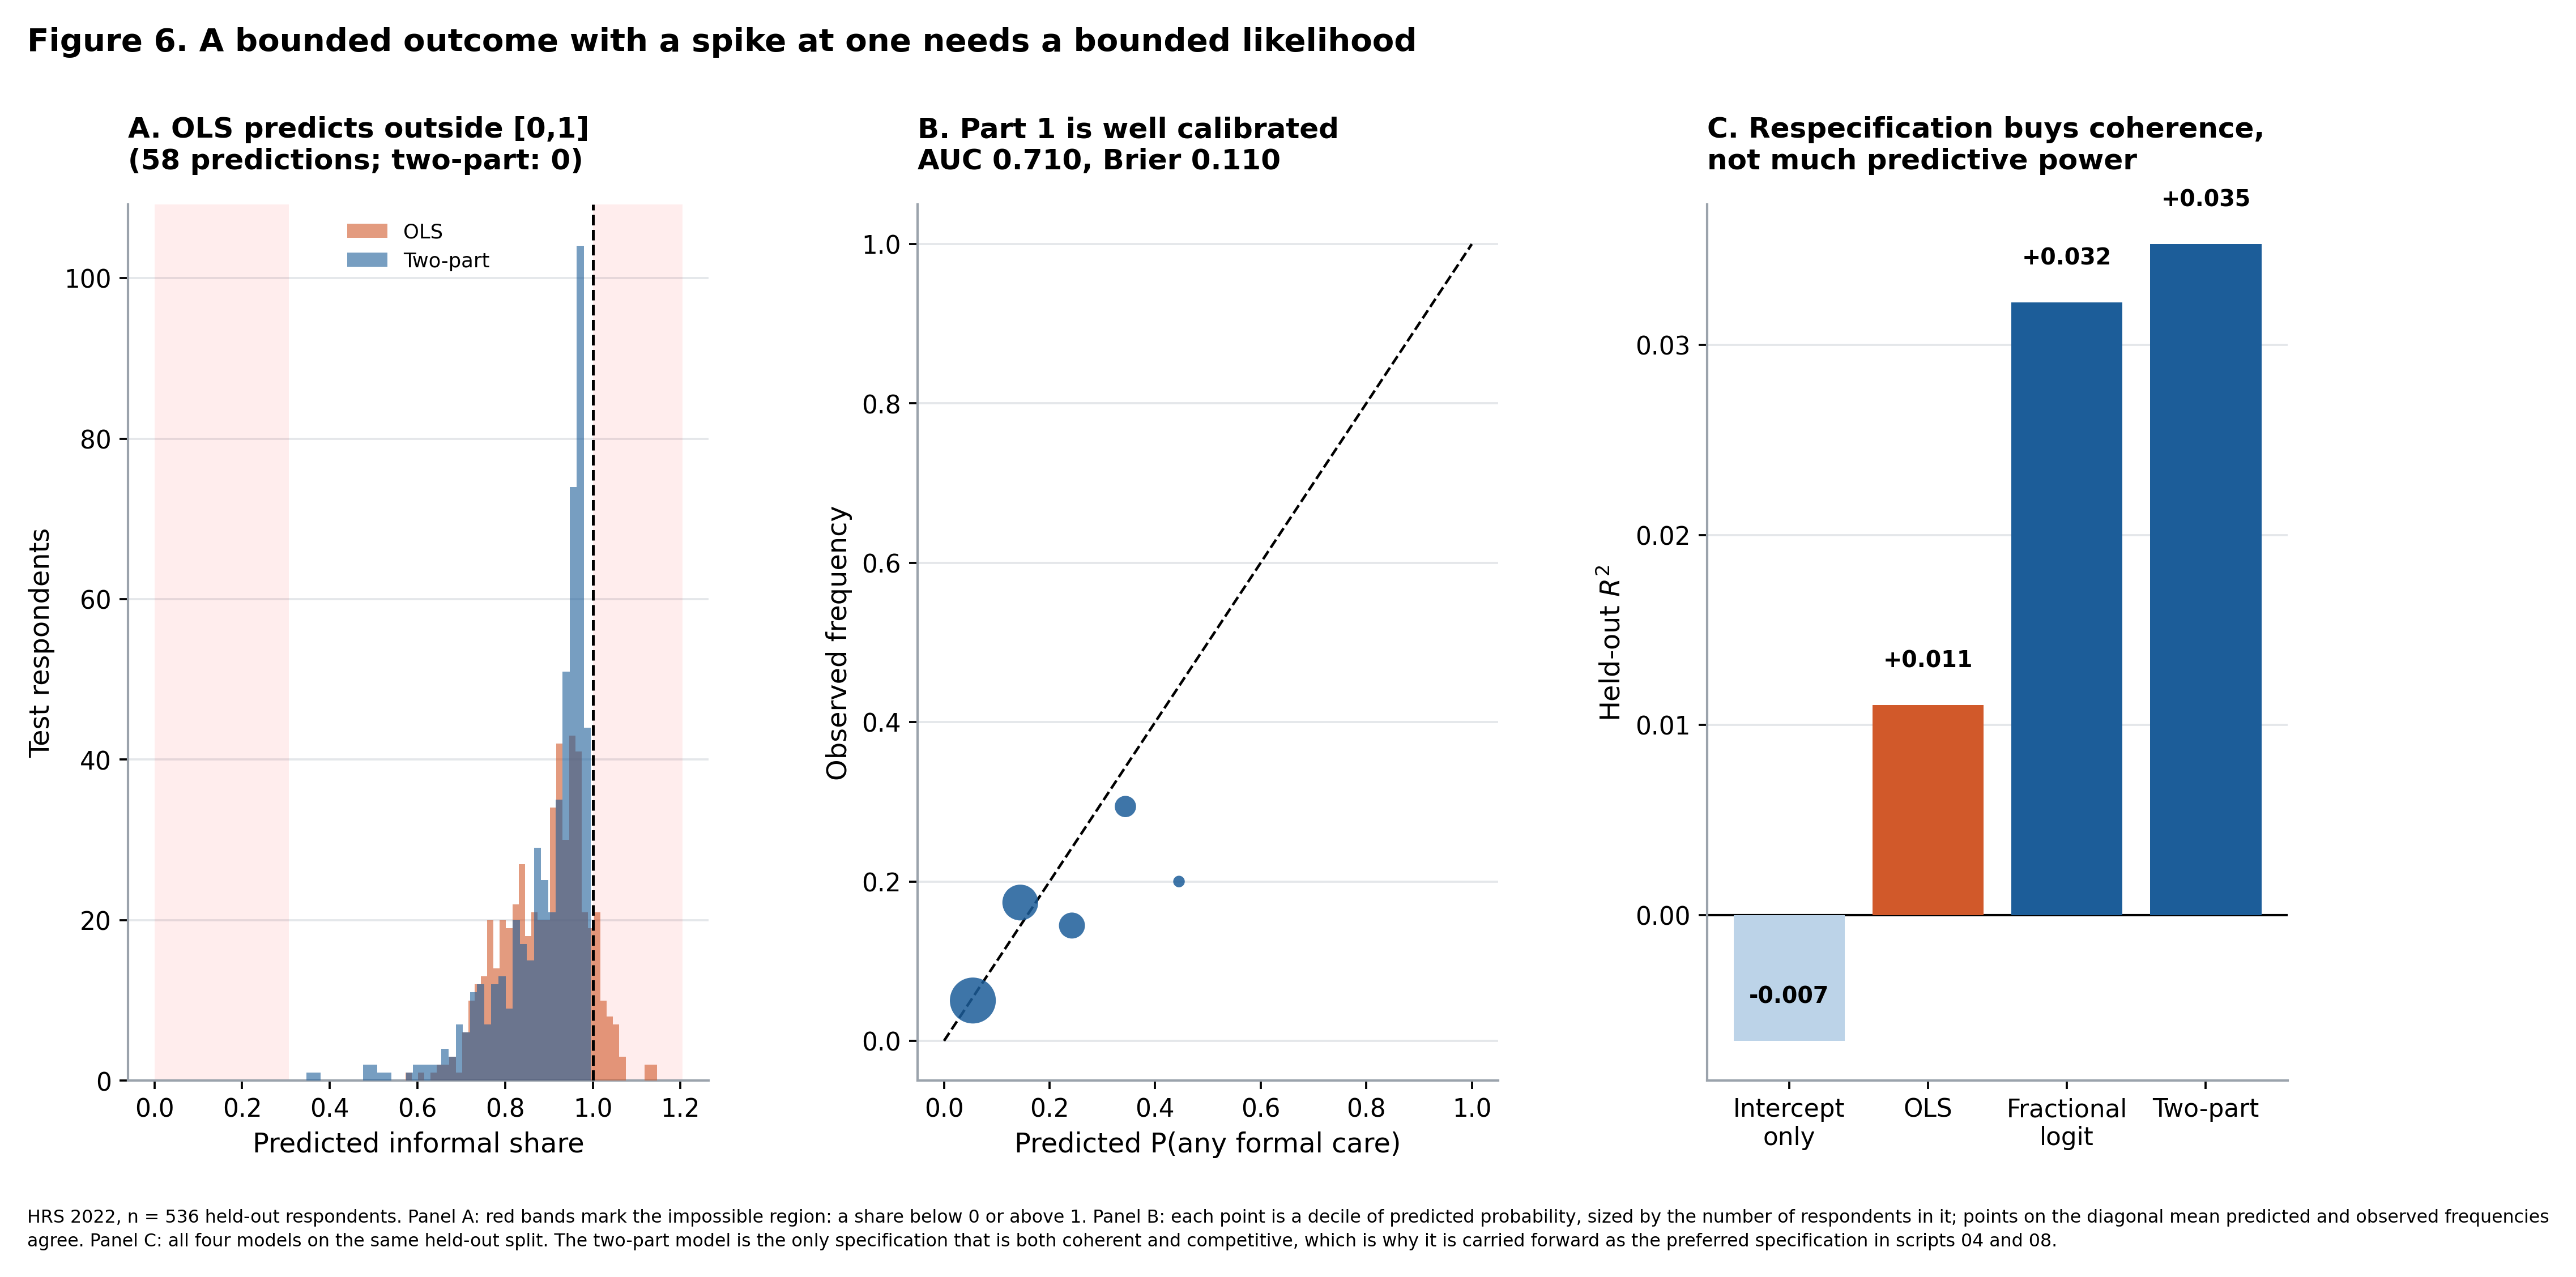
\includegraphics[width=0.80\linewidth]{figures/f06_two_part.png}
\caption{A bounded outcome with a spike at one requires a bounded likelihood.
Red bands in the left panel mark the impossible region.}
\label{fig:twopart}
\end{figure}

\subsection*{Need and living arrangement interact}

Litwak's model is the only one of the three that requires an interaction, and
main-effects models assume it away before they start. Fourteen pre-specified
interaction tests were run, of which five are significant at the 5\% level
against roughly 0.7 expected by chance. The strongest is between total care
hours and living alone ($\beta = -0.032$, $P = 0.005$): among people living
alone, rising care intensity pushes arrangements toward formal provision far
more sharply than it does for people living with a partner. Independently, the
pairwise SHAP interaction decomposition ranks the same pair first out of 630
(Fig.~\ref{fig:inter}). Two methods with different assumptions selecting the
same interaction is stronger evidence than either alone.

The within-group need gradients are also revealing. The slope of the informal
share on ADL count is $-0.011$ ($P = 0.0006$) among respondents living with a
partner and $-0.014$ ($P = 0.031$) among those living with a relative, but a
flat and insignificant $-0.005$ ($P = 0.52$) among those living alone. For
people who live alone, additional functional limitation does not
systematically bring formal care in---which is the opposite of what an
equity-satisfying system would produce.

\begin{figure}[tbhp]
\centering
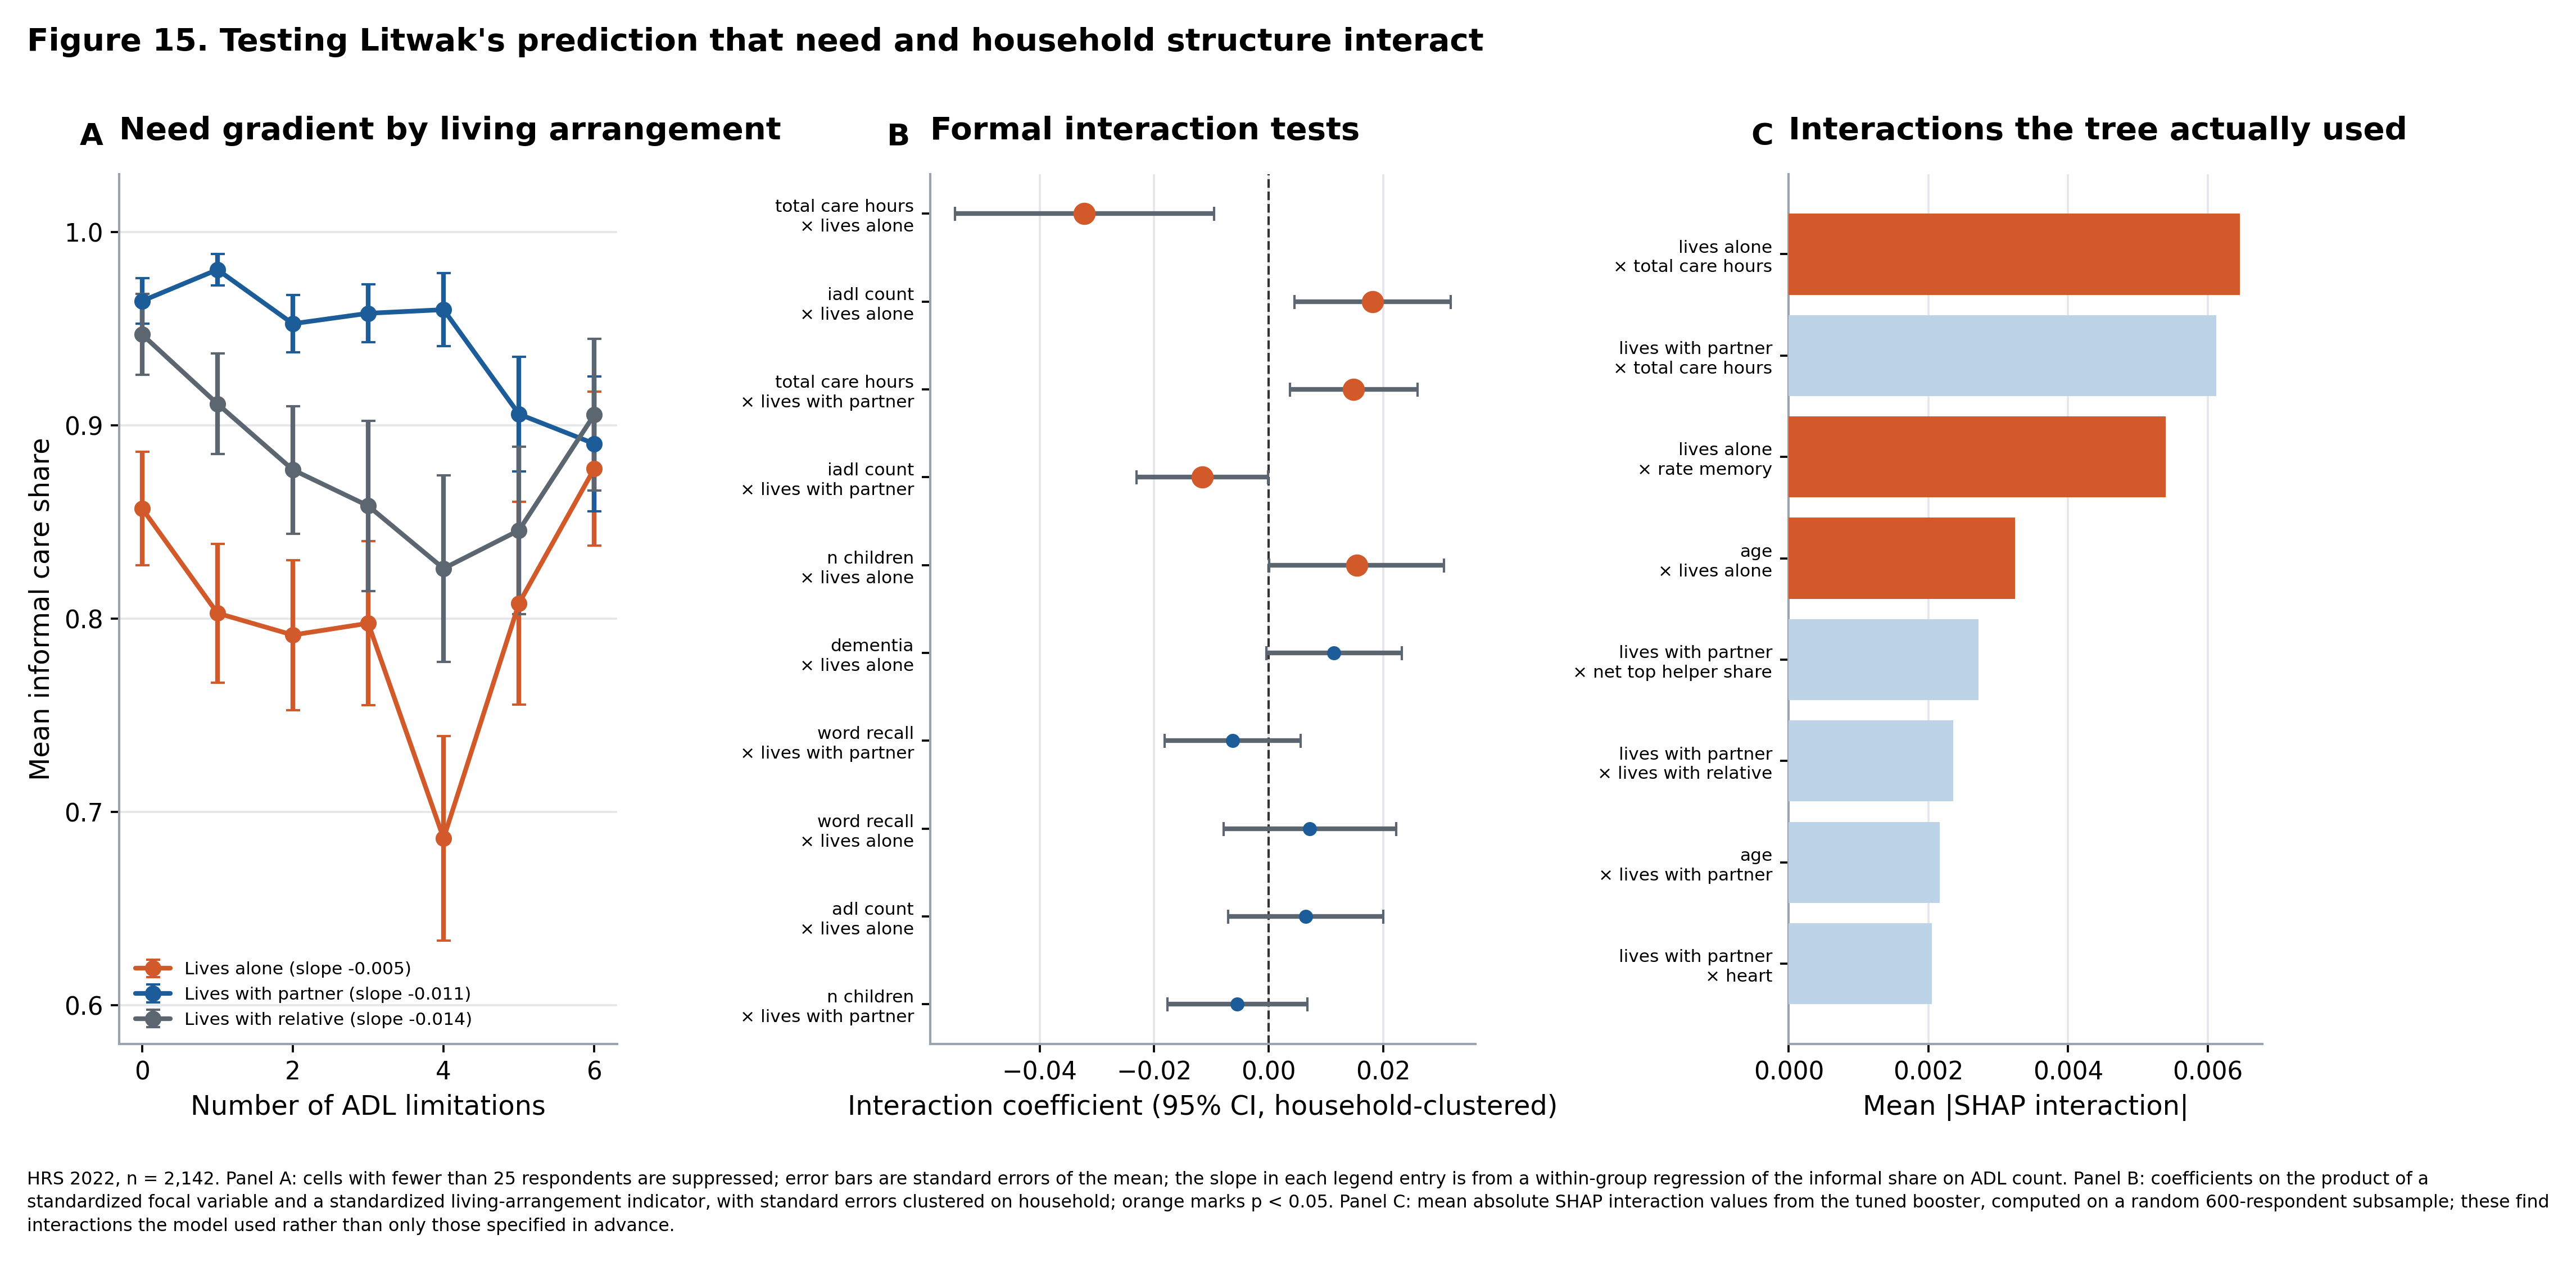
\includegraphics[width=0.80\linewidth]{figures/f15_interaction_grid.png}
\caption{Testing the prediction that need and household structure interact.
Panel B shows pre-specified interaction coefficients with household-clustered
standard errors; panel C shows interactions the tree actually used.}
\label{fig:inter}
\end{figure}

\begin{table}[tbhp]
\centering
\caption{The five interactions significant at the 5\% level, of fourteen
pre-specified tests. Standard errors are clustered on household.}
\label{tab:inter}
\small
\begin{tabular}{llr}
\toprule
Focal variable & Moderator & $\beta$ ($P$) \\
\midrule
Total care hours & Lives alone         & $-0.032$ ($0.005$) \\
IADL count       & Lives alone         & $+0.018$ ($0.009$) \\
Total care hours & Lives with partner  & $+0.015$ ($0.009$) \\
IADL count       & Lives with partner  & $-0.012$ ($0.048$) \\
Number of children & Lives alone       & $+0.015$ ($0.048$) \\
\bottomrule
\end{tabular}
\end{table}

Table~\ref{tab:inter} lists them. The pattern is coherent rather than scattered:
care intensity and instrumental-activity need both interact with living
arrangement, and the two living-arrangement moderators carry opposite signs, as
they must if they are picking up the same underlying contrast from opposite
ends. With fourteen tests roughly 0.7 significant results would be expected by
chance, so five is well above the multiple-testing floor, though the individual
$P$-values should not be read as if each test stood alone.

\subsection*{A two-tier leakage failure}

Treating each respondent's helper set as an ego network yields nine structural
features. Two are the outcome re-encoded---\texttt{net\_any\_formal} is true
exactly when the informal share is below one---and including them lifts
cross-validated $R^2$ from 0.087 to 0.644. Removing them is not sufficient.
Four more, the kin-composition features, are zero exactly when nobody in the
roster is family, which is the same event as the informal share being zero: 94
respondents have zero distinct kin types and their mean informal share is
exactly 0.000. That second tier still yields $R^2 = 0.553$, and is invisible to
a correlation scan because each feature looks unremarkable in isolation. With
both tiers removed, the genuinely exogenous network features move $R^2$ from
0.0874 to 0.0864---that is, not at all.

The general point is that the outcome is \emph{constructed from} the helper
roster, so every roster-derived feature is downstream of it. The operative test
is not whether a feature correlates with the outcome but whether it could have
been known without knowing the outcome.

\subsection*{Automated cross-national harmonization}

Extending this design across countries requires mapping HRS variables onto their
counterparts in sister surveys, and that mapping is where such projects stall:
the English Longitudinal Study of Ageing calls the dressing item
\texttt{headldr} where HRS calls it \texttt{SG014}. Embedding the variable
\emph{descriptions} and matching on cosine similarity reconstructs the crosswalk
at 71.4\% top-1 and 78.6\% top-5 accuracy against all 403 ELSA derived
variables, where random selection would score 0.2\%.

The failure pattern is the useful part. On ten ADL and IADL items the matcher
gets nine right. On four items where the two studies measure the same construct
with different instruments it gets zero right, and does so confidently---matching
``number of years in school'' to ELSA's count of adults in the benefit unit at
0.82 similarity. However, all four errors fall in the bottom four by
\emph{similarity margin}, the gap between the best and second-best candidate. A
rule that auto-accepts high-margin matches and routes the rest to a human would
have caught every error while accepting 71\% of the crosswalk automatically. A
matcher that is wrong 29\% of the time is not deployable; one that is wrong 29\%
of the time and knows which 29\% is.

\section*{Discussion}

Across five model families, three outcome specifications, survey weighting,
household-clustered validation, network features and an interaction analysis,
the substantive conclusion does not move: household composition determines who
absorbs the cost of long-term care, and clinical need barely registers. That
stability is the most useful thing this quantity of robustness work can report.

The equity reading is direct. Andersen's criterion holds that need should drive
utilization and that enabling resources driving it instead is the signature of
inequity. Here enabling structure dominates, and the interaction results
sharpen the point: among people living alone---who by construction have no
household member to absorb care---additional functional limitation does not
reliably bring formal provision in. The households with the least internal
capacity to absorb care are not being compensated by the market.

Four limitations bound it. The analysis is cross-sectional and single-country;
the outcome's degeneracy caps achievable accuracy for every model class, so
absolute performance is not a verdict on the methods; living arrangement is not
randomly assigned and is plausibly a consequence of care need as much as a
determinant of how it is met; and the nursing-home weighting artefact means
institutionalized respondents belong in a separate model. Nothing here is a
causal estimate.

\section*{Agentic Analysis}

An AI assistant (Claude, Anthropic) was used throughout, for notebook
scaffolding, figure code, and prose drafting, working from my research design
and my reading of the HRS codebooks. The interaction was iterative rather than
delegated: I specified the analysis, reviewed every output, and executed all
code. Three episodes are worth recording because they illustrate different
failure modes.

\paragraph{What I accepted.} The assistant proposed the missing-indicator
strategy over native NaN handling in gradient boosting, with the argument about
SHAP contamination reproduced in the Data section. I accepted it after
confirming the missingness pattern was non-random, and it survives as a
methodological commitment of the paper.

\paragraph{What I rejected.} An early version of the harmonization experiment
scored 100\% for all three matchers. Inspecting the ground-truth table showed
why: the HRS labels had been written as paraphrases of the ELSA wording, so the
lexical baseline was matching on words the assistant had itself introduced.
Rewriting with verbatim codebook labels and expanding the candidate set from 39
health variables to all 403 dropped accuracy to 71\% and made the experiment
informative. A confirmatory result had been manufactured by a badly constructed
test, and nothing in the output signalled it.

\paragraph{Where the AI failed.} The leakage described above was
\emph{introduced} by assistant-written feature-engineering code and was not
flagged in it. The first tier was caught quickly. The second tier---the
kin-composition features---survived one round of review and was found only by
asking of each feature what event makes it zero. Notably, the assistant then
also mislabelled the corrected feature set as ``safe'' in its own commentary,
which is the specific danger: fluent, well-commented code carrying an error that
the fluency conceals. A separate episode in the companion project produced a
plausible narrative about household clustering inflating cross-validated
performance; the data showed no such effect, and the narrative had been written
before the number was computed.

\paragraph{A third failure, in presentation rather than analysis.} A later
revision produced figures whose titles were silently cut off in the saved PNG
files. The cause was not obvious from the code, which looked correct: the SHAP
plotting library mutates the active Matplotlib figure and its global style
settings as a side effect, so a title set before that call falls outside the
saved bounding box and caption text renders in an invisible color. The
assistant's first two attempted fixes addressed symptoms, adjusting padding and
layout parameters, and neither worked. The eventual fix was structural, which is
to render each panel to its own file and composite them afterward. The general
shape of the failure is the same as the leakage: fluent code that looks right,
producing output that is wrong in a way the code does not reveal.

\paragraph{What this implies for the workflow.} AI assistance shifts the
location of the work rather than removing it. Writing code became fast;
verifying that the code answered the intended question became the binding
constraint. The three failures above share a structure: in each case the
assistant produced output that was internally consistent and externally wrong,
and in each case the error surfaced only when I asked what a quantity
\emph{meant} rather than whether the code ran. That is a poor fit for automated
checking and a good fit for domain knowledge, which is an argument for keeping
the researcher in the loop at the level of interpretation rather than
syntax. Every result in this paper that I would defend orally is one where I
traced the computation back to the codebook myself.

\Endparasplit

\section*{Analyses not shown here}

Four figures and three tables appear in this paper. The pipeline produces sixteen
figures and nineteen tables. The twelve figures held back are not weaker versions
of the five included; they answer adjacent questions, and each carries a
self-contained caption in the repository, numbered to match the script that
writes it.

Two extend the description: who the helpers are across all 4,481 records, and
the unconditional need gradient before it is split by living arrangement. Two
concern model comparison: importance rankings across four methods, and the
weight and clustering diagnostics behind the claim that weighted and unweighted
models describe different populations. Two concern the care networks, as ego
graphs and as derived feature distributions, and one pairs the feature-block
ablation with the final model's SHAP summary. Two support the crosswalk: the
embedding space the matcher searches, and the per-item confidence margins that
make its four errors identifiable in advance. The last decomposes the strongest
interaction as a partial-dependence surface.

The seventeen omitted tables are the numeric backing for results stated in prose
here, from the sample-construction audit and descriptives through the coefficient
and cross-validation comparisons to the ablation ladder, the crosswalk with its
per-item similarities, and the SHAP interaction pairs.

\section*{Materials and Methods}

All code is available at \url{https://github.com/alannap27/qss45-informal-care}
as ten numbered Python scripts with shared utilities in \texttt{code/utils.py}
and figure layout rules in \texttt{code/figstyle.py}. HRS microdata are not
redistributable and require free registration at \url{https://hrs.isr.umich.edu};
the repository documents the rebuild path. Analyses used Python 3.10 with pandas,
scikit-learn, statsmodels, XGBoost, SHAP and NetworkX; exact versions are pinned
in \texttt{requirements.txt}. Random seeds are fixed throughout.

\dataavail{Every figure and table in this paper, and the twelve figures and
sixteen tables not shown, are regenerated by \texttt{bash run\_all.sh} once the
HRS files are in place. Script 00, which rebuilds the analysis file from the raw
Section G helper records, is excluded from that command because its input cannot
be redistributed.}

\acknow{I thank Prof.\ Herbert Chang for guidance on the analysis design, and
the QSS 45 cohort for feedback on an earlier version of these results.}

\showacknow

\bibliography{qss45}

\end{document}
